\chapter{Conservación del ambiente de ejecución}

En este trabajo, se argumenta que las descripciones de los ambientes computacionales son necesarias para la reproducción del experimento. Además, la información debe ser la suficiente para comparar y detectar las diferencias entre el ambiente original y el reproducido.

Dado que las imágenes Docker son ambientes aislados e independientes, asumimos que los componentes de software dentro del contenedor si están relacionados al experimento y no existen componentes relacionados a otros experimentos dentro del mismo contenedor.
Por esta razón, se asegura que las anotaciones no presentarán ruido de otras herramientas o dependencias asociadas, causadas por entremezclar la ejecución de otros experimentos con otros requisitos computacionales en el mismo contenedor.
Para realizar una anotación automática de los paquetes instalados, se propone e implementa un sistema de anotación automático. El sistema requiere el nombre de una imagen existente en un repositorio de DockerHub y los datos del repositorio Git que almacena el archivo Dockerfile. 

Los pasos asociados del sistema anotación:
\begin{enumerate}
	\item Consultar al repositorio de imágenes Docker los metadatos de la imagen. 
	\item Anotar los metadatos utilizando la ontología propuesta.
	\item Descargar cada una de las capas asociadas a la imagen Docker.
	\item El sistema anotador consulta a Clair, Clair monta cada una de capas de la imagen, detecta los componentes de software instalados a través el sistema de paquete.
	\item Obtener la información desde Clair y anotar los datos obtenidos por Clair según la ontología.
	\item Guardar los datos en una base de datos RDF.
\end{enumerate} 

%----------------------------------
% 4.1 Semantic models
%----------------------------------
\section{Modelos semánticos}\label{s4.1}
     
En \cite{santana2017reproducibility}, los autores proponen \emph{The Workflow Infrastructure Conservation Using Semantics ontology (WICUS)}. WICUS es ontología OWL2 (Web Ontology Language) que implementa la conceptualización de los principales dominios de la infraestructura computacional. Estos son: Hardware, Software, Workflow y recursos de computo.
Los autores definen que los workflows científicos requieren un conjunto de componentes de software, y los investigadores deben conocer cómo desplegar estos componentes para lograr ambiente equivalente.\todo[inline]{describe un p[oco mejor tu contribución con la ontología, tiene que quedar claro que esto también es una contribución, sobre todo el detalle más fino que logras}
Considerando que la ontología está relacionada con nuestro trabajo, se utiliza algunas clases y relaciones desde la ontología WICUS descriptas a continuación:

\begin{description}
	\item [DeploymentPlan:]  Un plan de despliegue está compuesto de todos los pasos. Y el plan de despliegue le permite entender al investigador cuáles fueron los pasos requeridos para construir el ambiente computacional.
	\item [DeploymentStep:] Cada paso de despliegue es representado por una línea de comando que realiza la instalación, descarga o configuración del ambiente. La información se obtiene desde el archivo DockerFile
	\item [SoftwareComponent:] Es un componente de software instalado sin una versión específica. 
\end{description} 

La ontología propuesta define el recurso \texttt{dockerpedia:SoftwarePackage} como una subclase de \texttt{wicus:SoftwareComponent} para definir los componentes instalados por el gestor de paquetes del sistema operativo u otro.
Cada \texttt{wicus:SoftwareComponent} tiene una relación \texttt{dockerpedia:hasVersion} o \texttt{dockerpedia:isVersionOf} que muestra la versión del software instalado.
El recurso \texttt{dockerpedia:PackageVersion} puede estar afectado por vulnerabilidades representadas por el recurso \texttt{dockerpedia:SoftwareVulnerability}. Y las versiones que reparan la vulnerabilidad se encuentran representadas por \texttt{dockerPedia:SecurityRevision}.
Una imagen Docker se representa por \texttt{dockerpedia:SoftwareImage} y sus capas por el recurso \texttt{dockerpedia:ImageLayer}. Los paquetes instalados en la imagen están relacionado por \texttt{vocab:ContainsSoftware} con su imagen.
Finalmente, el sistema operativo es representado por el recurso \texttt{dockerpedia:OperatingSystem} y cada imagen y capa de la imagen está asociado al recurso.
Con estas clases, podemos representar las capas que componen la imagen del ambiente computacional, los paquetes de software presentes en la imagen y en cada una de sus capas y además las vulnerabilidades asociadas a los paquetes.
Desde el punto de los investigadores, la representación de las descripciones con esta ontología permite un formato claro para consultar y almacenar los datos.
Una versión completa de la ontología se encuentra disponible en nuestros repositorios \footnote{\url{https://github.com/dockerpedia/ontology/}} y la versión resumida se observa en la figura ~\ref{fig:ontology}. 

\begin{figure}[t]
  \centering
    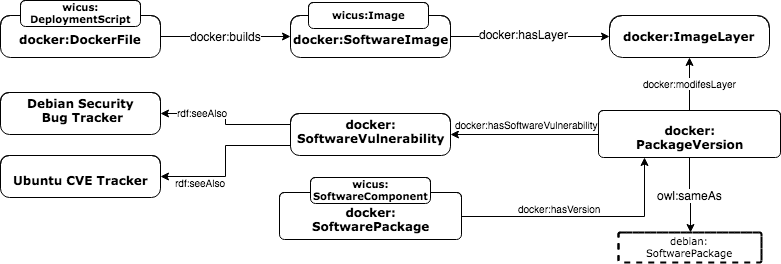
\includegraphics[width=1\textwidth]{Figures/dockerOntologyBasic.png}
      \caption{Ontología resumida para DockerPedia.}
     \label{fig:ontology}

\end{figure}

%----------------------
% 4.2 Annotator
%-----------------------
\section{Anotador}\label{s4.2}

El servicio de anotación propuesto cuenta con una interfaz REST para recibir el nombre y la versión de la imagen Docker relacionada con el experimento científico. 
Para almacenar e interactuar con los datos el sistema de anotación utiliza a Apache Jena~\footnote{\url{https://jena.apache.org/}}. Apache Jena es un framework Java, de código abierto basado en la licencia Apache 2.0 \footnote{\url{http://www.apache.org/licenses/LICENSE-2.0}} para la construcción de aplicaciones de Web Semántica y Datos Enlazados. El sistema anotador construye los triples relacionados con el experimento, imagen, capas, componentes de software y vulnerabilidades y se envían usando la API de Apache Jena que serializa los triples utilizando formatos populares como RDF/XML o Turtle.
Es importante remarca que la arquitectura permita la utilización de otras herramienta en caso que Apache Jena no cumpla con los requerimientos de escalabilidad.

El sistema anotación realiza dos tipos de anotaciones: Componentes de software y pasos de construcción.


%--------------------------------------------
% 4.2.1 Building steps annotations
%---------------------------------------------
\subsection{Anotaciones de los pasos de construcción}\label{s4.2.1}

Anotamos el plan de despliegue (Deployment Plan) usando dos métodos. El primer método obtiene los pasos desde el archivo Dockerfile entregado por el usuario, esto permite obtener los pasos y la ubicación de archivo en el repositorio. 
Usando este método se asegura la reconstrucción del ambiente debido a que cualquier archivo necesario por Dockerfile se encuentra en el repositorio Git.
Sin embargo, un usuario puede construir una imagen sin compartir el archivo Dockerfile. En ~\cite{DBLP:conf/semweb/OsorioAV18a} se reporta que sólo el 30\% de las imágenes Docker en DockerHub vincula su archivo Dockerfile. 
Por lo tanto, si no existe información del Dockerfile el sistema anotación utiliza el manifiesto de la imagen Docker. Sin embargo, si el usuario no comparte su repositorio con los archivos no podemos asegurar la reproducibilidad por la falta del código o configuración y la información se guarda para referencia del investigar.
Respecto al manifiesto,  según \footnote{\url{https://docs.docker.com/registry/spec/manifest-v2-2/}} el manifiesto de la imagen provee la configuración y el conjunto de las capas y pasos de construcción de la imagen.
 
 
Algunos atributos relevantes del manifesto son:

\begin{description}
	\item [name:] \textit{string} nombre de la imagen
	\item [tag:] \textit{tag} versión de la imagen
	\item [architecture:] \textit{string} arquitectura del servidor en cuál la imagen ha sido construido. Esta información actualmente no es utilizada por Docker.
	\item [fsLayers:] \textit{array} lista de las capas que componente la imagen.
		La estructura contiene los siguiente campos:
		\begin{description}
			\item [blobSum:] es un identificador utilizando una función de hash sha256 para cada capa de la imagen 
		\end{description}
	\item [history]: \textit{array} Es una lista de datos históricos no estructurados para la compatibilidad con la v1. Contiene ID de la capa de imagen y el ID de las capas principales de la capa. El historial es una estructura que consta de los siguientes campos:
	\begin{description}
		\item[v1Compatibility]:  \textit{string} V1Compatibilidad es la información de compatibilidad de V1 en bruto. Esto contiene el objeto JSON que describe la V1 de esta imagen. Una V1Compatibilidad es una estructura que consta de los siguientes campos:
		
		\begin{description}
			\item [Id:] \textit{string} ID de la capa utilizando hash sha256			\item [Parent:] \textit{string} ID de la capa madre utilizando hash sha256
				\item [ContainerConfig:] \textit{string} El comando que construyó la capa
		\end{description}
	\end{description}
\end{description}



%--------------------------------------------
% 4.2.2 Software Components annotations
%---------------------------------------------
\subsection{Anotaciones de componentes de software}\label{s4.2.2}

La descripción de los componentes de software es fundamental para realizar cuantificar la similitud entre dos o más ambientes computacionales.
Un enfoque común para detectar los componentes de software guardar o detectar los comandos que realizan la instalación de software. Por ejemplo, la figura \ref{lst:tensorflow} muestra los comandos para instalar los componentes de la imagen TensorFlow. 
\begin{figure*}
	\begin{lstlisting}[caption={Ejemplo de instalación de dependencias para la imagen TensorFlow},label={lst:tensorflow},language=bash]
apt-get install -y --no-install-recommends \
        build-essential \
        curl \
        libfreetype6-dev \
        libhdf5-serial-dev \
        libpng12-dev \
        libzmq3-dev \
        pkg-config \
        python \
        python-dev \
        rsync \
        software-properties-common \
        unzip	
\end{lstlisting}

\end{figure*}


El enfoque detectaría los componentes: \verb|build-essential|, \verb|curl|, \verb|libfreetype6-dev|, \verb|libhdf5-serial-dev|, \verb|libpng12-dev|, \verb|libzmq3-dev|, \verb|pkg-config|, \verb|python|, \verb|python-dev|, \verb|rsync|, \verb|software-properties-common| y  \verb|unzip|. Sin embargo, este enfoque no obtiene información sobre las versiones o las dependencias del software. Utilizando el  enfoque propuesto, se puede terminar que el línea anterior instala 184 paquetes.



Otro enfoque  para lograr la anotación de los componentes de software es utilizar los gestores de paquetes del sistema. Los gestores que paquetes se clasifican en dos tipos: gestor de paquetes del tipo sistema y general:

\begin{description}
	\item  [Gestor de paquetes de sistema:] son aquellos vinculados al sistema operativo (e.g., apt de familia Debian, yum de familia RedHat).
	\item [Gestor de paquetes generales:] son aquellos externos que normalmente son utilizados para instalar componentes de software de terceros ó un lenguaje especifico (e.g., python, conda, npm). Por ejemplo, conda es un sistema paquete frecuentemente utilizado por investigadores al estar relacionado con Jupyter Notebook.
\end{description}


Es por ello que se utiliza Clair que fue introducido en la sección  \ref{sec:clair}, éste permite la detección componentes de software y vulnerabilidades dentro de una imagen de un contendor.
En este trabajo se utiliza Clair para detectar los componentes de software debido a que (i) no se necesita ejecutar el contenedor para detectar los componentes de software, (ii) no necesita instalar componentes de software extras dentro de la imagen y por lo tanto no se añade ruido al sistema, (iii) permite la extensión a otro tipo de sistema de contenedores como Singularity\footnote{\url{https://www.sylabs.io/docs/}}~\cite{kurtzer2017singularity} y (iv) el análisis es realizado por capas, lo que permite re usar análisis de otras capas ya analizadas.

Además, como prueba de generalidad se extiende Clair para detectar los paquetes instalados por Conda en la imagen.  
Sin embargo, Clair no cumple totalmente las necesidades para solucionar los problemas de anotación dado que Clair no considera múltiples detectores en la misma imagen y los componentes de software detectados son generados a partir de diferencias.
Por ejemplo, si se supone una imagen que está compuesta de dos capas: A y B donde A es padre de B y Clair presenta dos detectores \texttt{Alpha} y \texttt{Beta}. Donde el detector \texttt{Alpha} detecta componentes de software en el archivo \verb|/etc/a| y  \texttt{Beta} detecta componentes de software en el archivo \verb|/etc/b|. Si en la capa A, \texttt{Alpha} lista el software \verb|1| en \verb|/etc/a| y \texttt{Beta} lista \verb|2| en  \verb|/etc/b|. Y luego, en la capa B, \texttt{Beta}  lista \verb|2| y \verb|3| en  \verb|/etc/b|. El resultado de las diferencias será: 

\begin{enumerate}
	\item A añadió a \verb|1| y \verb|2|. Dado que observa el componentes de software en \verb|/etc/a| y \verb|/etc/b|
	\item  B añadió a \verb|3| y se mantuvo \verb|2| dado que observan en \verb|/etc/b|. Y se removió \verb|1| porque no hay archivo \verb|/etc/a|
\end{enumerate}

Pero si \verb|/etc/a| no tuvo cambios, el archivo no se ve incluye en la capa hija. Y no significa que el \verb|1| fuese removido. 
La casual del problema es que Clair añade y remueve paquetes sin considerar los detectores que detectaron los componentes de software. 
Consecuentemente, en esta propuesta se utiliza una copia del proyecto Clair que discrimina según el sistema de paquete que instaló el componente para permitir múltiples sistemas de paquetes de la imagen. El proyecto se encuentra disponible en el repositorio de DockerPedia \footnote{\url{https://github.com/dockerpedia/clair}}.

En la figura  \ref{fig:packages-pegasus} se muestra triples de algunos de los paquetes instalado en la imagen de un workflow construido con Pegasus, en la figura \ref{fig:vulnerability-pegasus} se muestra sus vulnerabilidades.
\begin{figure}[t]
    \hspace*{-4cm}   
    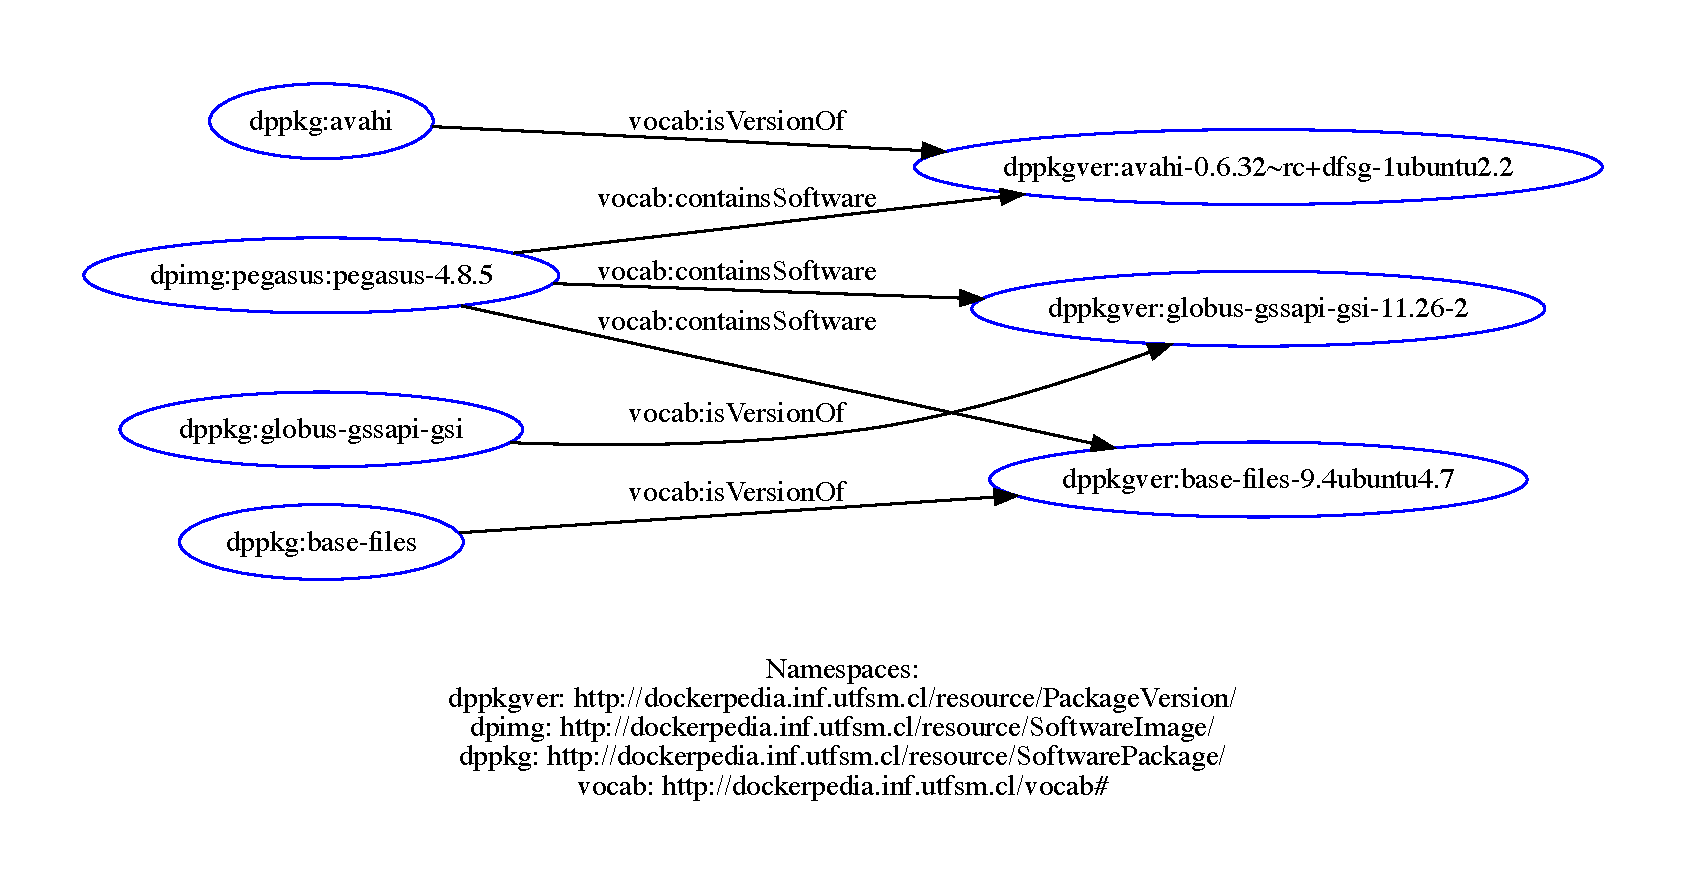
\includegraphics[width=1.3\textwidth]{Figures/packages}
     \caption[Paquetes de la imagen Pegasus]{Ejemplo de triples que muestran los componentes de software de la imagen Pegasus}
    \label{fig:packages-pegasus}
      
\end{figure}

\begin{figure}[t]
    \hspace*{-4cm}   
    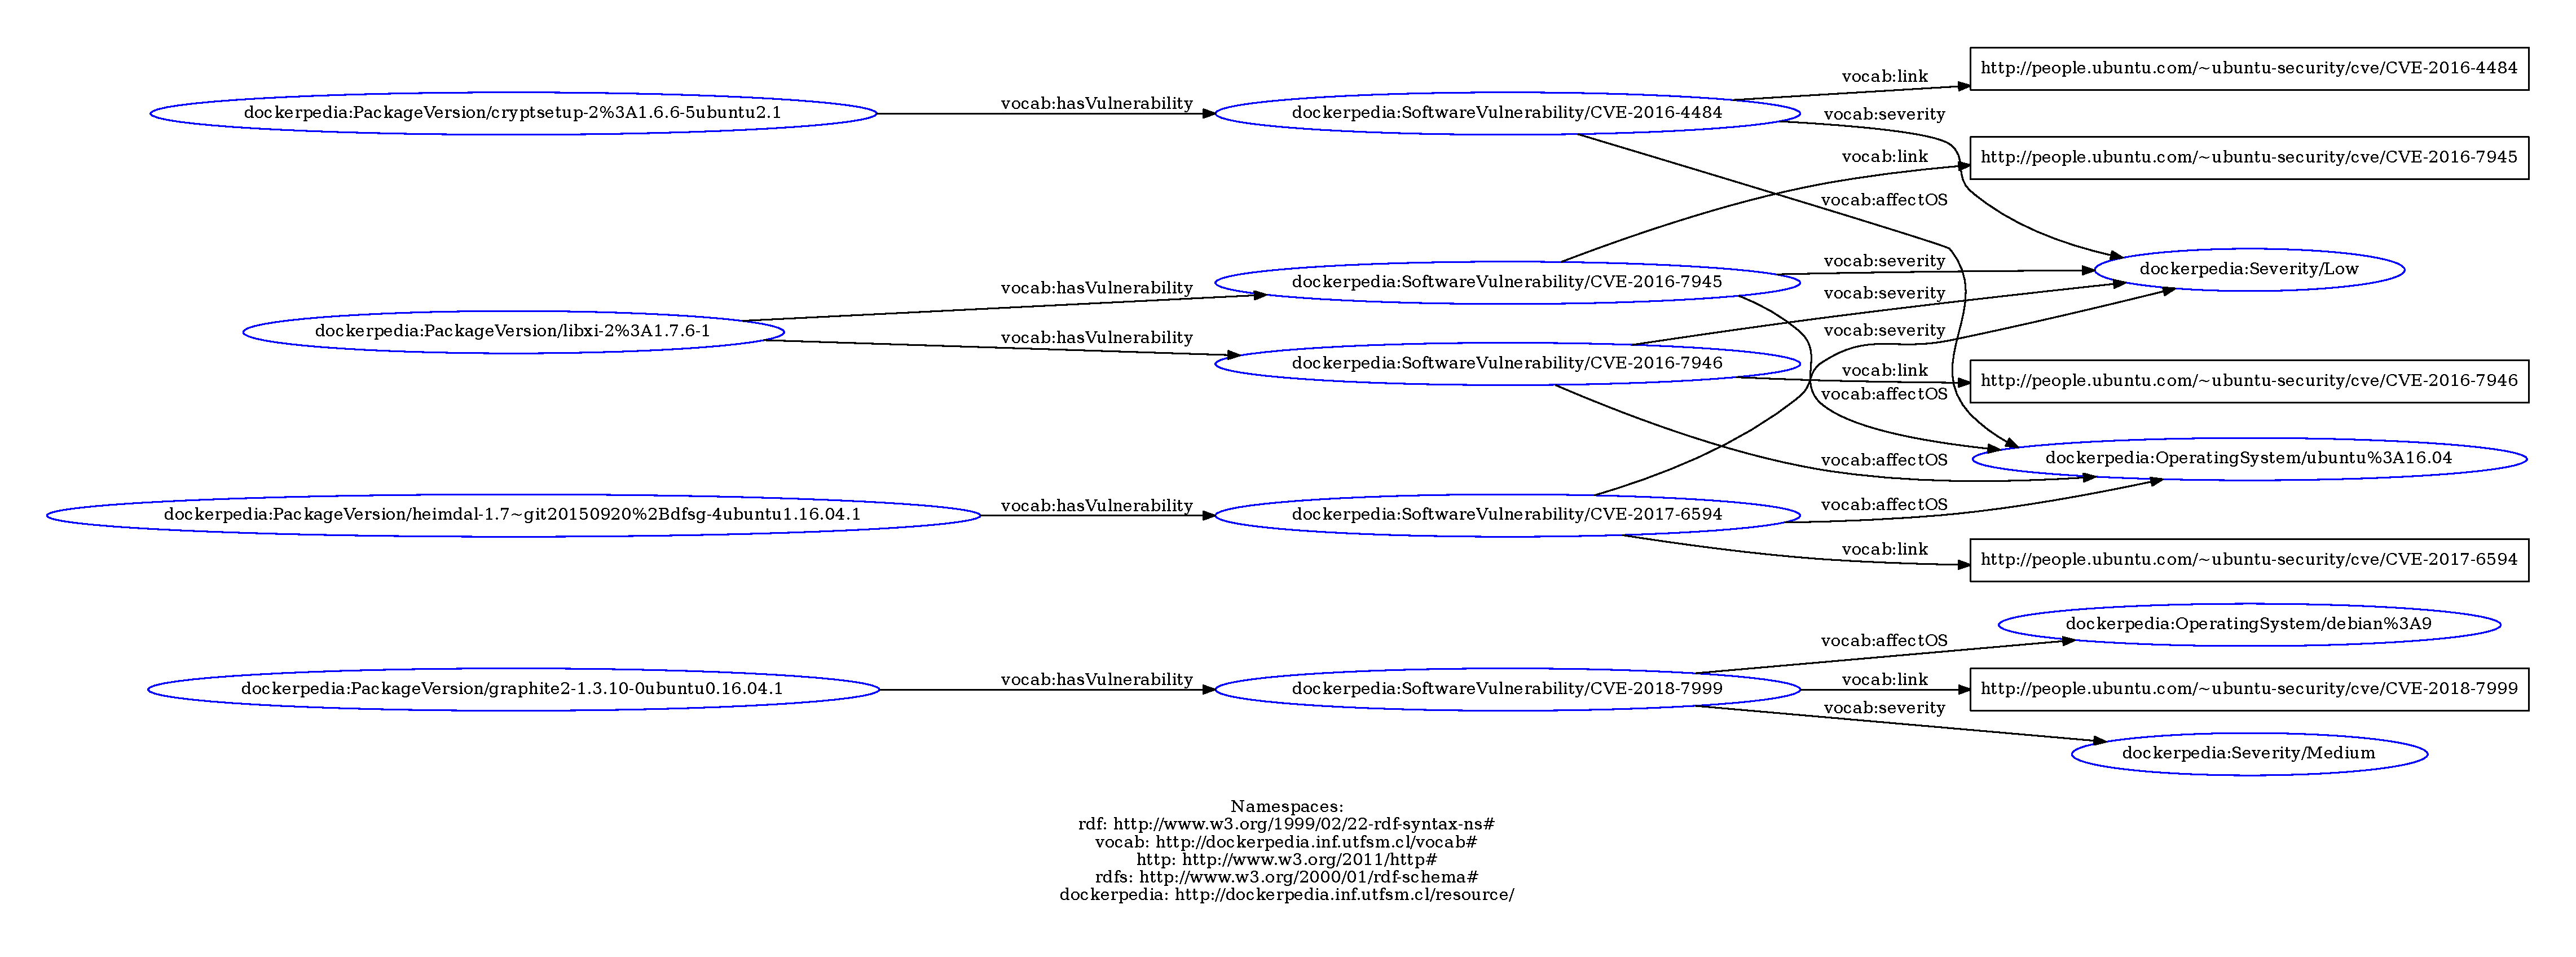
\includegraphics[width=1.3\textwidth]{Figures/packages-vuln}
      \caption[Paquetes y vulnerabilidades de la imagen Pegasus]{Vulnerabilidades y paquetes vulnerables de la imagen Pegasus}
    \label{fig:vulnerability-pegasus}
\end{figure}

\todo[inline]{termina los capítulos con un resumen de lo que has hecho, e introduciendo el siguiente, para que el lector siga con la curiosidad de qué viene después. Tienes que pensar también que el lector primero irá a la introducción del capítulo, después a las conclusiones de ese mismo capítulo y luego mirará el contenido si le interesa, tal y como pasa con el documento en general y como dice el libro Trees Maps and Theorems}